% =============================================================================
% tmp.tex --- quick scratch doc for the two Tier 1/2 architecture diagrams.
% Build with:  pdflatex tmp.tex
% =============================================================================
\documentclass[11pt,letterpaper]{article}

% --- Core encoding + fonts ---
\usepackage[utf8]{inputenc}
\usepackage[T1]{fontenc}

% --- Math packages ---
\usepackage{amsmath}
\usepackage{amssymb}
\usepackage{amsthm}
\usepackage{amsfonts}
\usepackage{bm}

% --- Layout / figures / tables ---
\usepackage{graphicx}
\usepackage{booktabs}
\usepackage{geometry}
\geometry{margin=1in}
\usepackage{xcolor}

% --- hyperref LAST ---
\usepackage[colorlinks=true,linkcolor=blue,citecolor=blue,urlcolor=blue]{hyperref}

% No custom commands in the body --- use full \bm{\theta}, \mathcal{L}, \mathbb{R}
% directly so the build is robust to preamble-load failures.

\title{UltraClear --- Tier 1 (Macro) and Tier 2 (Micro) Diagram Notes}
\author{tmp scratch}
\date{\today}

\begin{document}
\maketitle

% =============================================================================
\section*{Tier 1: Macro-environment FOMAML training}
% =============================================================================

\begin{figure}[h]
  \centering
  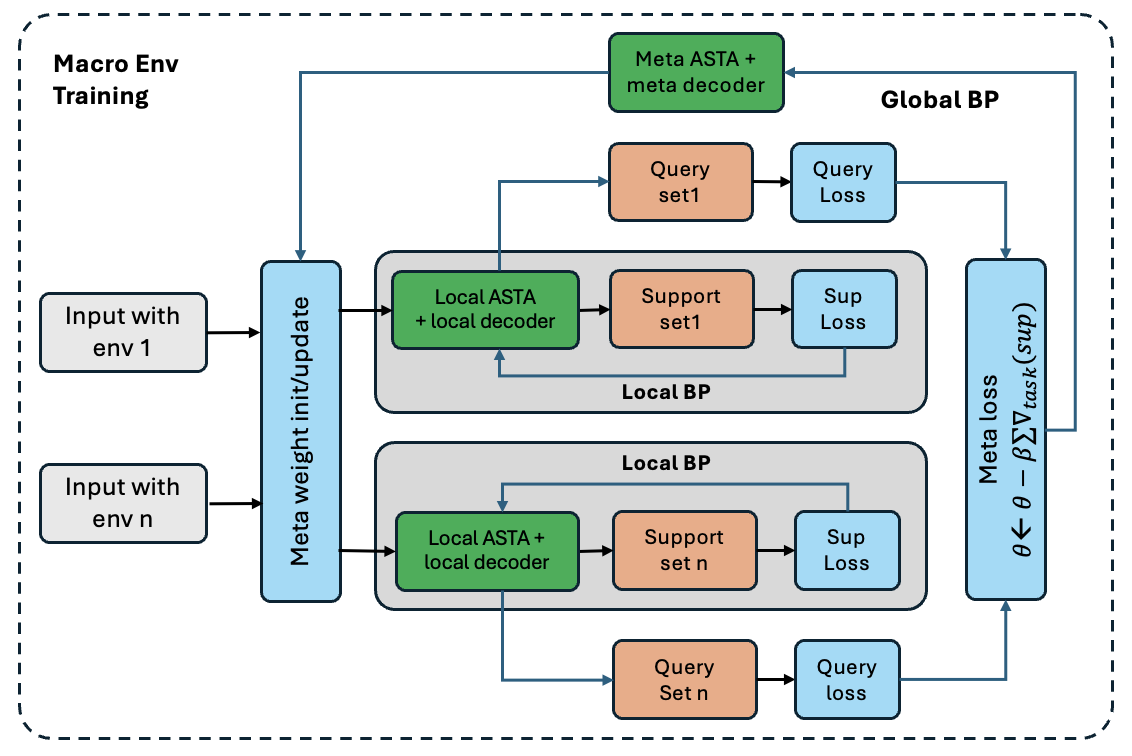
\includegraphics[width=0.95\linewidth]{figures/macro.png}
  \caption{Tier~1 FOMAML training over deployment environments.
  Each environment's input is processed by a per-task branch
  (Local ASTA + local decoder) initialized from the shared
  meta-parameters, adapted on a support set via the inner loop
  (Local BP), and evaluated on a query set. The query losses
  across environments are aggregated into a meta-loss that
  updates the shared meta-parameters via Global BP, so the
  meta-learner produces an initialization from which few-shot
  adaptation generalizes across environments.}
  \label{fig:macro}
\end{figure}

The Tier~1 FOMAML loop treats each deployment environment
$e \in \{1, \dots, N\}$ as a meta-task. For every task, the
shared meta-parameters $\bm{\theta}$ are cloned and adapted on a
$K$-shot support set $\mathcal{S}_e$ via $J$ inner gradient
steps with learning rate $\alpha$:
$\bm{\theta}_e^{(j+1)} \leftarrow \bm{\theta}_e^{(j)} - \alpha \nabla_{\bm{\theta}_e^{(j)}}
\mathcal{L}_{\mathrm{task}}(f_{\bm{\theta}_e^{(j)}}(\mathcal{S}_e))$.
We use first-order MAML (FOMAML) --- the second-order term is
dropped to keep the inner loop cheap and stable. The adapted
per-task model $\bm{\theta}_e^{(J)}$ is then evaluated on a
$Q$-sample query set $\mathcal{Q}_e$, and the meta-loss
$\mathcal{L}_{\mathrm{meta}}(\bm{\theta}) = \sum_{e} \mathcal{L}_{\mathrm{task}}(f_{\bm{\theta}_e^{(J)}}(\mathcal{Q}_e))$
is back-propagated through the inner loop to update the shared
initialization: $\bm{\theta} \leftarrow \bm{\theta} - \beta \nabla_{\bm{\theta}}
\mathcal{L}_{\mathrm{meta}}(\bm{\theta})$. At test time, the same
procedure is applied to a new unseen environment using only $K$
labeled support shots --- no online fine-tuning is required
beyond the inner-loop adaptation.

% =============================================================================
\section*{Tier 2: Micro-condition FiLM disentanglement}
% =============================================================================

\begin{figure}[h]
  \centering
  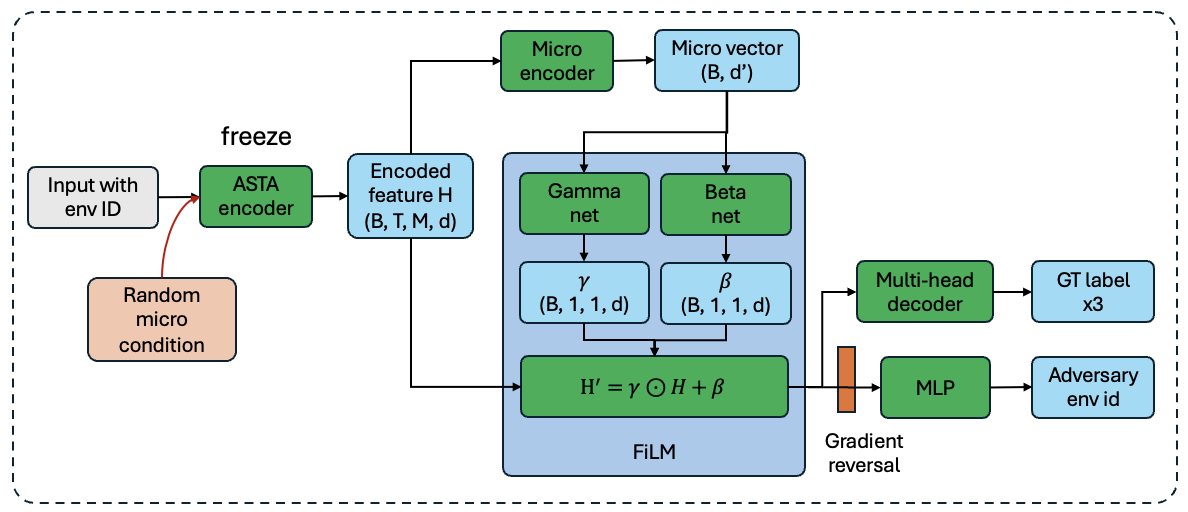
\includegraphics[width=0.95\linewidth]{figures/micro.png}
  \caption{Tier~2 FiLM-based micro-condition disentanglement.
  The pretrained ASTA encoder is frozen and acts as a fixed
  feature extractor producing per-cell features
  $\bm{H} \in \mathbb{R}^{B \times T \times M \times d}$. A small
  micro encoder pools $\bm{H}$ into a compact condition vector
  $\bm{c} \in \mathbb{R}^{B \times d'}$, which two small networks
  map into per-feature multiplicative and additive scales
  $\bm{\gamma}$ and $\bm{\beta}$. The FiLM-conditioned features
  $\bm{H}' = \bm{\gamma} \odot \bm{H} + \bm{\beta}$ feed a
  multi-head decoder for the supervised task and, through a
  gradient-reversal layer, an adversary that tries to recover
  the macro environment identity. The reversal forces $\bm{H}'$
  to be informative for the task but uninformative about the
  macro environment, yielding a disentangled micro
  representation.}
  \label{fig:micro}
\end{figure}

The Tier~2 pipeline runs on top of the Tier~0/1 ASTA encoder
$f_\theta$, which is \emph{frozen} so the gradient-reversal
adversary cannot push the encoder itself toward a constant and
kill the location-relevant signal. The frozen encoder produces
per-cell features $\bm{H} = f_\theta(\bm{X}) \in \mathbb{R}^{B \times T \times M \times d}$,
which a small micro encoder $h_\phi$ pools into a compact
condition vector $\bm{c} \in \mathbb{R}^{B \times d'}$. Two
linear networks then produce per-feature multiplicative and
additive scales
$\tilde{\bm{\gamma}}(\bm{c}), \tilde{\bm{\beta}}(\bm{c}) \in \mathbb{R}^{B \times d}$
(reshaped to $(B,1,1,d)$ and broadcast over $T, M$), and FiLM
modulates the features via
$\bm{H}' = (\mathbf{1} + \tilde{\bm{\gamma}}(\bm{c})) \odot \bm{H} + \tilde{\bm{\beta}}(\bm{c})$.
The networks are initialized so that $\bm{\gamma} = \mathbf{1}$
and $\bm{\beta} = \mathbf{0}$ at the start of training,
i.e.\ FiLM is the identity at init. The conditioned features
$\bm{H}'$ feed a multi-head decoder for the three supervised
targets (NLOS identification, signal restoration, location) and,
through a gradient-reversal layer that negates the upstream
gradient by $\lambda$, an adversary $D_\xi$ that attempts to
recover the macro environment identity from $\bm{H}'$. The total
loss is
$\mathcal{L}_{\mathrm{Tier2}} = \mathcal{L}_{\mathrm{sup}} - \lambda \mathcal{L}_{\mathrm{adv}}$,
where the $-\lambda$ sign comes from the gradient reversal: the
adversary is trained to predict the env id, but the signal
flowing back into the FiLM and micro encoder \emph{opposes}
that prediction, so $\bm{H}'$ ends up informative for the task
but uninformative about the macro environment.

\end{document}
